\section{\texorpdfstring{Kết quả nghiên cứu}{result}}
%Mô tả ngắn gọn các kết quả nghiên cứu, thực nghiệm. Bàn luận về điểm mạnh, điểm yếu của mô hình được xây dựng trong luận văn. So sánh kết quả thu được trong quá trình nghiên cứu, thực nghiệm của đề tài và đối chiếu với kết quả nghiên cứu, thực nghiệm của các tác giả khác một cách khách quan. Nêu lên điểm nổi bật, khác biệt của luận văn đối với các nghiên cứu khác.

Trong phần này, tất cả các mô hình được miêu tả đều được huấn luyện trên thiết bị đồ họa NVIDIA V100 và bộ xử lý Intel Xeon với 24GB bộ nhớ truy xuất ngẫu nhiên. Các thí nghiệm tạo sinh hình ảnh và đanh giá dữ liệu đều được thực hiện trên thiết bị máy tính cá nhân sử dụng thiết bị đồ họa RTX 3070, bộ xử lý Intel Core I5 8600K và 32GB bộ nhớ truy xuất ngẫu nhiên.

\subsection{Các kết quả trên tập dữ liệu GRID}

\begin{table}[h]
    \centering
    \begin{tabular}{c | c | c | c | c}
    \hline 
    \multicolumn{5}{c}{GRID}\\
    \hline 
    \textbf{$\mathcal{L}_{landmark}$} & \textbf{$\mathcal{L}_{pix}$} & \textbf{$\mathcal{L}_{gans-dis}$} & \textbf{$\mathcal{L}_{gans-landmark}$} & \textbf{$\mathcal{L}$}\\
    \hline
    $4.9200 \times 10^{-4}$ & $4.1575 \times 10^{-2}$ & $0.9964$ & $7.6990 \times 10^{-2}$ & $1.4892$\\
    \hline
    \end{tabular}
    \caption{Các giá trị mất mát của mạng khi hội tụ tại vòng lặp thứ 8}
    \label{table:grid_loss}
\end{table}

\begin{figure}[H]
    \centering
    \includegraphics[width=15cm]{./content/materials/grid_examples-landmark.png}
    \caption{Kết quả tạo sinh cột mốc gương mặt trên tập GRID}
\end{figure}

\begin{figure}[H]
    \centering
    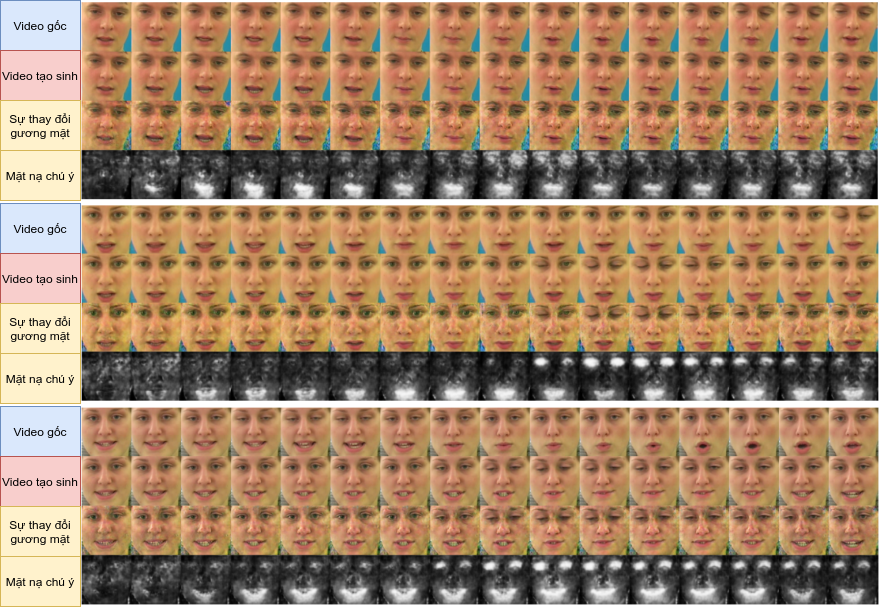
\includegraphics[width=15cm]{./content/materials/grid_examples-face.png}
    \caption{Kết quả tạo sinh gương mặt theo giọng nói trên tập GRID}
\end{figure}

\subsection{Các kết quả trên tập dữ liệu LRW}

Do tập dữ liệu có khối lượng dữ liệu lớn hơn tập GRID nhiều lần và dữ liệu không được chuẩn hóa tốt như tập dữ liệu GRID. Huấn luyện mạng trên tập LRW cũng khó hội tụ hơn và không cho kết quả tốt như tập GRID. Với tập dữ liệu LRW, thời gian huấn luyện là 9 giờ 30 phút cho mỗi vòng lặp qua dữ liệu (tính trên thiết bị đồ họa NVIDIA V100). Mạng hội tụ và cho kết quả tốt nhất sau 25 vòng lặp. Tại thời điểm hội tụ, các hàm mất mát trên mạng có giá trị:

\begin{table}[h]
    \centering
    \begin{tabular}{c | c | c | c | c}
    \hline 
    \multicolumn{5}{c}{LRW}\\
    \hline 
    \textbf{$\mathcal{L}_{landmark}$} & \textbf{$\mathcal{L}_{pix}$} & \textbf{$\mathcal{L}_{gans-dis}$} & \textbf{$\mathcal{L}_{gans-landmark}$} & \textbf{$\mathcal{L}$}\\
    \hline
    $2.012 \times 10^{-4}$ & $6.8502 \times 10^{-2}$ & $0.6931$ & $5.2412 \times 10^{-2}$ & $1.4306$\\
    \hline
    \end{tabular}
    \caption{Các giá trị mất mát của mạng khi hội tụ tại vòng lặp thứ 25}
    \label{table:lrw_loss}
\end{table}

\begin{figure}[H]
    \centering
    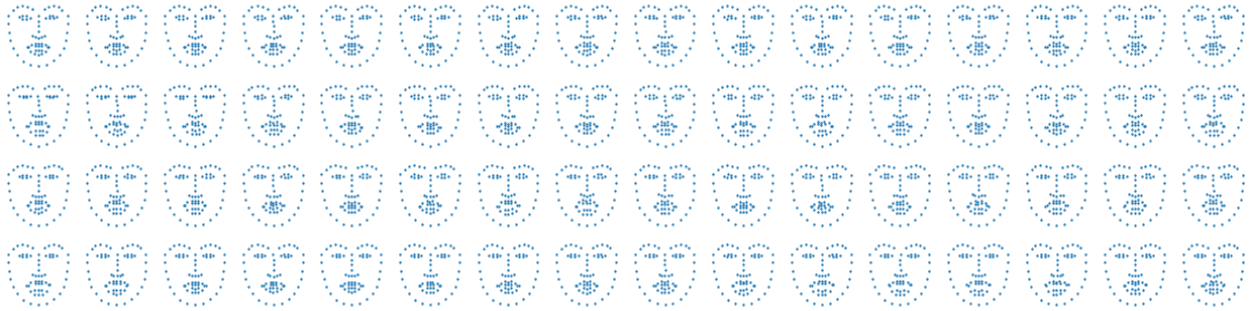
\includegraphics[width=15cm]{./content/materials/lrw_examples-landmark.png}
    \caption{Kết quả tạo sinh cột mốc gương mặt trên tập LRW}
\end{figure}

Hình sau thể hiện kết quả tạo sinh video khi cho mô hình tạo sinh ảnh trên tập kiểm thử với 3 trường hợp: ảnh mẫu được chuẩn hóa tốt, ảnh đầu vào bị lệch, và ảnh đầu vào được quay một bên mặt.

\begin{figure}[H]
    \centering
    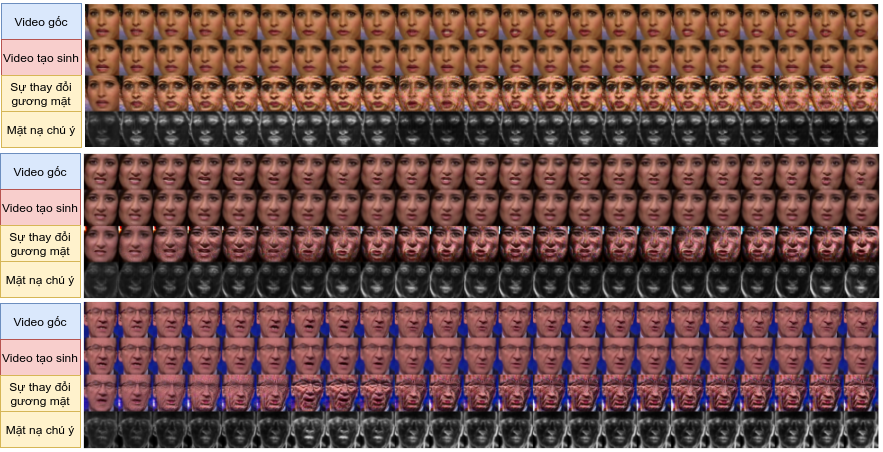
\includegraphics[width=15cm]{./content/materials/lrw_examples-frontal.png}
    \caption{Kết quả tạo sinh gương mặt theo giọng nói trên tập LRW, trường hợp ảnh đầu vào là hình ảnh chiếu thẳng mặt người nói, mặt người được canh bốn góc, mũi nằm ở giữa khung hình}
\end{figure}

\begin{figure}[H]
    \centering
    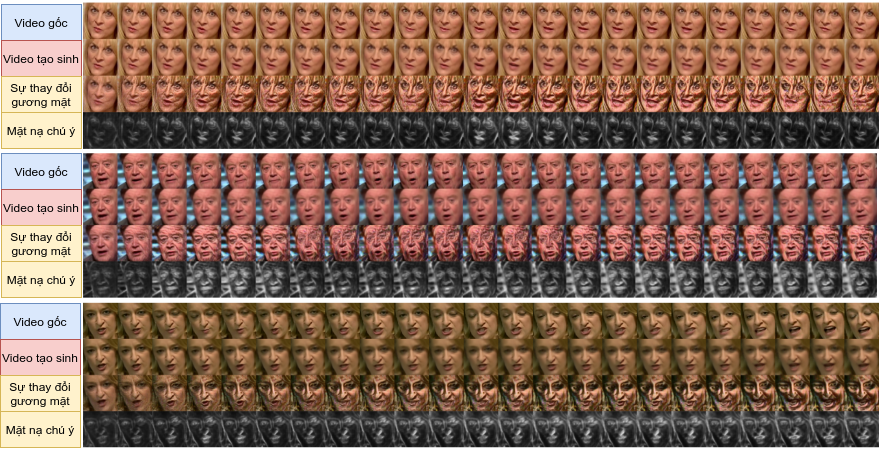
\includegraphics[width=15cm]{./content/materials/lrw_examples-miss_aligned.png}
    \caption{Kết quả tạo sinh gương mặt theo giọng nói trên tập LRW, trường hợp ảnh đầu vào là hình ảnh bị lệch, mặt người nằm ở 1 phía trên khung hình}
\end{figure}

\begin{figure}[H]
    \centering
    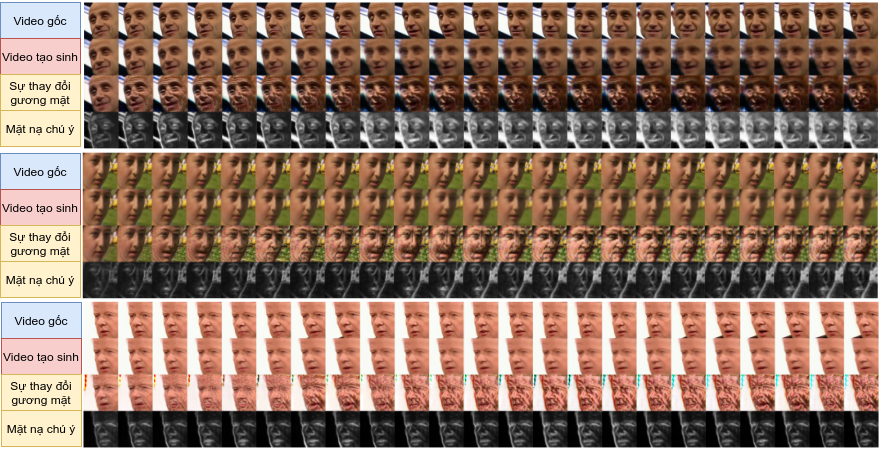
\includegraphics[width=15cm]{./content/materials/lrw_examples-half_face.png}
    \caption{Kết quả tạo sinh gương mặt theo giọng nói trên tập LRW, trường hợp ảnh đầu vào là hình ảnh lệch hẳn về một bên mặt}
\end{figure}

Hình ảnh trên cho thấy, mạng cho kết quả tốt nhất khi tạo sinh ảnh có chứa mặt người mẫu được chụp theo hướng chính diện, mặt người được chuẩn hóa tốt.
